\documentclass{article}


\usepackage{arxiv}

\usepackage[utf8]{inputenc} % allow utf-8 input
\usepackage[T1]{fontenc}    % use 8-bit T1 fonts
\usepackage{hyperref}       % hyperlinks
\usepackage{url}            % simple URL typesetting
\usepackage{booktabs}       % professional-quality tables
\usepackage{amsfonts}       % blackboard math symbols
\usepackage{nicefrac}       % compact symbols for 1/2, etc.
\usepackage{microtype}      % microtypography
\usepackage{lipsum}		% Can be removed after putting your text content
\usepackage{amsmath} 
\usepackage{amssymb}
\usepackage{graphicx}
\usepackage{epstopdf}
\usepackage{url}
\usepackage{setspace}
\usepackage{amsthm}
\usepackage{mathrsfs}
\usepackage{enumitem}
\usepackage{parskip}
\usepackage{IEEEtrantools}
\usepackage{mathtools}
\usepackage{tensor}
\usepackage{yfonts}
\usepackage{dsfont}
\usepackage{braket}

\usepackage{pgfplots}
\pgfplotsset{compat=1.15}

\usetikzlibrary{arrows}

\definecolor{zzttqq}{rgb}{0.6,0.2,0}
\definecolor{uuuuuu}{rgb}{0.26666666666666666,0.26666666666666666,0.26666666666666666}
\definecolor{xdxdff}{rgb}{0.49019607843137253,0.49019607843137253,1}

\newtheorem{theorem}{Theorem}[section]
\newtheorem{lemma}[theorem]{Lemma}
\newtheorem*{lemma*}{Lemma}
\newtheorem{prop}[theorem]{Proposition}
\newtheorem{corollary}[theorem]{Corollary}
\newtheorem{defn}[theorem]{Definition\rm}
\newtheorem{conjecture}[theorem]{Conjecture}
\newtheorem{remark}{\it Remark\/}
\newtheorem{example}{Example}
\newtheorem{fact}{Fact}

\newcommand{\st}{\ensuremath{:}}% such that
\newcommand{\ie}{\emph{i.e.} }
\newcommand{\eg}{\emph{e.g.} }
\newcommand{\cf}{\emph{cf.} }
\newcommand{\ra}{\rightarrow}
\newcommand{\la}{\leftarrow}
\newcommand{\lra}{\longrightarrow}
\newcommand{\lla}{\longleftarrow}
\newcommand{\lbracket}{\left(}
\newcommand{\rbracket}{\right)}


\newcommand{\al}{\alpha}
\newcommand{\w}{\omega}
\newcommand{\W}{\Omega}
\newcommand{\m}{\mu}
\newcommand{\n}{\nu}
\newcommand{\e}{\epsilon}
\newcommand{\K}{K\"ahler }
\newcommand{\HK}{hyperk\"ahler }
\newcommand{\into}{\hookrightarrow}
\newcommand{\PP}{\mathbb{P}}
\newcommand{\RR}{\mathbb{R}}
\newcommand{\CC}{\mathbb{C}}
\newcommand{\QQ}{\mathbb{Q}}
\newcommand{\FF}{\mathbb{F}}
\newcommand{\ZZ}{\mathbb{Z}}
\newcommand{\NN}{\mathbb{N}}
\newcommand{\HH}{\mathbb{H}}
\newcommand{\vp}{\varphi}
\newcommand{\mcA}{\mathcal{A}}
\newcommand{\mcE}{\mathcal{E}}
\newcommand{\mcF}{\mathcal{F}}
\newcommand{\mcG}{\mathcal{G}}
\newcommand{\mcH}{\mathcal{H}}
\newcommand{\mcL}{\mathcal{L}}
\newcommand{\mcO}{\mathcal{O}}
\newcommand{\mfg}{\mathfrak{g}}
\newcommand{\mfh}{\mathfrak{h}}
\newcommand{\mft}{\mathfrak{t}}
\newcommand{\mc}[1]{\mathcal{#1}}
\newcommand{\mf}[1]{\mathfrak{#1}}

\newcommand{\pbrackets}[1]{\left( #1 \right)}
\newcommand{\bbrackets}[1]{\left[ #1 \right]}

\newcommand{\dbar}{\bar{\partial}}
\newcommand{\mrr}{\mu_{\mathbb{R}}}
\newcommand{\mcc}{\mu_{\mathbb{C}}}
\newcommand{\prr}{\phi_{\mathbb{R}}}
\newcommand{\pcc}{\phi_{\mathbb{C}}}

\DeclareMathOperator{\Lie}{Lie}
\DeclareMathOperator{\Aut}{Aut}
\DeclareMathOperator{\Tr}{Tr}
\DeclareMathOperator{\Image}{Im}
\DeclareMathOperator{\Ad}{Ad}
\DeclareMathOperator{\Diff}{Diff}
\DeclareMathOperator{\Vect}{Vect}
\DeclareMathOperator{\Sympl}{Sympl}
\DeclareMathOperator{\Span}{Span}
\DeclareMathOperator{\ind}{ind}
\DeclareMathOperator{\Td}{Td}
\DeclareMathOperator{\Ch}{Ch}
\DeclareMathOperator{\Ind}{Ind}
\DeclareMathOperator{\pt}{pt}
\DeclareMathOperator{\rk}{rk}
\DeclareMathOperator{\coker}{coker}
\DeclareMathOperator{\Pf}{Pf}
\DeclareMathOperator{\Vol}{Vol}
\DeclareMathOperator{\Res}{Res}

\DeclareMathOperator{\GL}{GL}
\DeclareMathOperator{\SO}{SO}
\DeclareMathOperator{\UU}{U}

\newcommand\restr[2]{{% we make the whole thing an ordinary symbol
		\left.\kern-\nulldelimiterspace % automatically resize the bar with \right
		#1 % the function
		\vphantom{\big|} % pretend it's a little taller at normal size
		\right|_{#2} % this is the delimiter
}}

\title{Hypertoric Manifolds}

\date{}	% Here you can change the date presented in the paper title
%\date{} 					% Or removing it

%\author{
%  David S.~Hippocampus\thanks{Use footnote for providing further
%    information about author (webpage, alternative
%    address)---\emph{not} for acknowledging funding agencies.} \\
%  Department of Computer Science\\
%  Cranberry-Lemon University\\
%  Pittsburgh, PA 15213 \\
%  \texttt{hippo@cs.cranberry-lemon.edu} \\
%% examples of more authors
%   \And
% Elias D.~Striatum \\
%  Department of Electrical Engineering\\
%  Mount-Sheikh University\\
%  Santa Narimana, Levand \\
%  \texttt{stariate@ee.mount-sheikh.edu} \\
%% \AND
%% Coauthor \\
%% Affiliation \\
%% Address \\
%% \texttt{email} \\
%% \And
%% Coauthor \\
%% Affiliation \\
%% Address \\
%% \texttt{email} \\
%% \And
%% Coauthor \\
%% Affiliation \\
%% Address \\
%% \texttt{email} \\
%}

\begin{document}
	\maketitle
	
	\begin{abstract}
		Notes on toric \HK manifolds.
	\end{abstract}
	
	\section{Cotangent Spaces to Extended Core Components}
	
	Let $M_{\lambda} = \pbrackets{\mu_{\RR}^{-1}(\lambda) \cap \mu_{\CC}^{-1}(0)}/K$ be a toric \HK manifold. Define
	\begin{equation*}
		\CC_{A} := \Set{ (z_{i}, w_{i}) \in \CC^{2n}\ | \ w_{i} = 0\, \text{if } i \in A, \text{ and } z_{i} = 0\, \text{if } i \not\in A } \cong \CC^{n} \subset \HH^{n}.
	\end{equation*}
	
	\begin{lemma}[\cite{Konno2002}]\label{cotangent:1}
		Let $M_{\lambda}$ be a toric \HK manifold. If $\mcE_{A}$ is non-empty, then its holomorphic cotangent bundle $T^{\ast}\mcE_{A}$ is contained in $M_{\lambda}$ as an open subset.
	\end{lemma}
	
	Fix a subset $A \subset \Set{1, \ldots, n}$, and define
	\begin{equation*}
		(x_{i}^{(A)}, y_{i}^{(A)}) :=
		\begin{cases}
			(z_{i}, w_{i}), \quad &\text{if } i \in A, \\
			(w_{i}, -z_{i}), \quad &\text{if } i \not\in A.
		\end{cases}
	\end{equation*}

	Then $x^{(A)} = (x_{1}^{(A)}, \ldots, x_{n}^{(A)})$ is a point in the vector space $\CC_{A}^{n}$, and $y^{(A)} = (y_{1}^{(A)}, \ldots, y_{n}^{(A)})$ is a point in the dual space $\pbrackets{\CC_{A}^{n}}^{\ast}$. That is, we identify the cotangent bundle $T^{\ast}\CC_{A}^{n}$ with $\HH^{n}$ as above.
	
	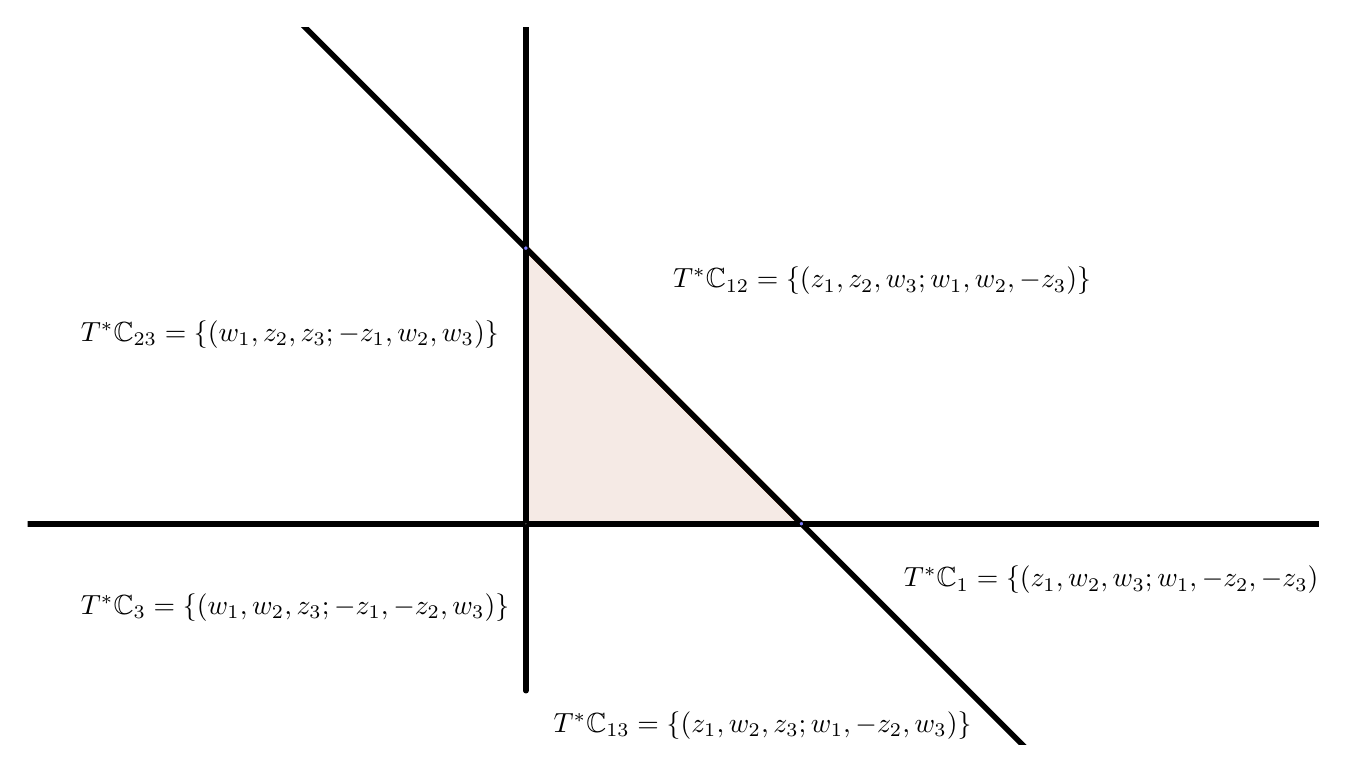
\begin{tikzpicture}[line cap=round,line join=round,>=triangle 45,x=1cm,y=1cm,scale=0.35]
		\clip(-18.076279350071736,-8) rectangle (28.778992688025916,18);
		\fill[line width=2pt,color=zzttqq,fill=zzttqq,fill opacity=0.10000000149011612] (10,0) -- (0,0) -- (0,10) -- cycle;
		\draw [line width=2pt,color=zzttqq] (10,0)-- (0,0);
		\draw [line width=2pt,color=zzttqq] (0,0)-- (0,10);
		\draw [line width=2pt,color=zzttqq] (0,10)-- (10,0);
		\draw (4.987051324183269,9.66247942901259) node[anchor=north west] {$T^{\ast}\mathbb{C}_{12} =\{(z_{1}, z_{2}, w_{3};w_{1}, w_{2}, -z_{3})\}$};
		\draw (-16.5,7.7288587527992325) node[anchor=north west] {$T^{\ast}\mathbb{C}_{23} =\{(w_{1}, z_{2}, z_{3};-z_{1}, w_{2}, w_{3})\}$};
		\draw (-16.5,-2.1914560208171174) node[anchor=north west] {$T^{\ast}\mathbb{C}_{3} =\{(w_{1}, w_{2}, z_{3};-z_{1}, -z_{2}, w_{3})\}$};
		\draw (0.6522562449167495,-6.4716909014277486) node[anchor=north west] {$T^{\ast}\mathbb{C}_{13} =\{(z_{1}, w_{2}, z_{3};w_{1}, -z_{2}, w_{3})\}$};
		\draw (13.366074254441164,-1.1826104506188444) node[anchor=north west] {$T^{\ast}\mathbb{C}_{1} =\{(z_{1}, w_{2}, w_{3};w_{1}, -z_{2}, -z_{3})\}$};
		\draw [line width=2pt,domain=-18.076279350071736:28.778992688025916] plot(\x,{(-100--10*\x)/-10});
		\draw [line width=2pt] (0,-6.05869737324383) -- (0,20.39547535639977);
		\draw [line width=2pt,domain=-18.076279350071736:28.778992688025916] plot(\x,{(-0-0*\x)/10});
		\begin{scriptsize}
			\draw [fill=xdxdff] (10,0) circle (2.5pt);
			\draw [fill=uuuuuu] (0,0) circle (2pt);
			\draw [fill=xdxdff] (0,10) circle (2.5pt);
		\end{scriptsize}
	\end{tikzpicture}

	\subsection{The Legendre Transform}
	
	In \cite{Konno2002}, Konno states that the proof of this lemma goes by an argument in \cite{Guillemin1994}, which itself is based on properties of the Legendre transform.
	
	\begin{lemma}[Section A1.3 of \cite{Guillemin1994}]
		Consider a smooth function of one variable
		\begin{equation*}
			f = f(x), \qquad -\infty < x < \infty.
		\end{equation*}
	
	Suppose that $f$ is strictly convex ($f^{\prime\prime}(x) > 0$ for all $x$). Then the four conditions are equivalent:
	\begin{enumerate}
		\item $f^{\prime}(x_{0}) = 0$ at some point $x_{0}$.
		\item $f$ has a local minimum at some point $x_{0}$.
		\item $f$ has a unique local minimum.
		\item $f(x)$ tends to $+ \infty$ as $x$ tends to $\pm \infty$.
	\end{enumerate} 
	\end{lemma}

	If $f$ has any one (and hence all four) of the above properties, we will say that $f$ is \emph{stable}.
	
	\section{Symplectic Cutting}
	
	\subsection{Compactifying the Extended Core}
	
	Let $S^{1}$ act on $M$ by rotating the cotangent fibres, that is, for $\tau \in S^{1}$,
	\[
		\tau \cdot [z; w] = [z; \tau w].
	\]
	This $S^{1}$-action is Hamiltonian, with moment map
	\[
		\Phi : M \lra (\RR)^{\ast}; \qquad [z:w] \longmapsto \frac{1}{2} \|w\|^{2}.
	\]
	Let $S_{A}^{1}$ denote the residual $S^{1}$-action on $M$ restricted to the extended core component 
	\[
		\mcE_{A} = \Set{ [z_{1}: \ldots z_{n}; w_{1}, \ldots, w_{n}] | w_{0} = 0 \text{ if } i \in A, \text{ and } z_{i} = 0 \text{ if } i \not\in A }.
	\]
	Now the \emph{global }$S^{1}$-action does not act on the cotangent fibres of $M$ as a subtorus of $T^{n}$, but it does when \emph{restricted} to each component of the extended core, $\mcE_{A}$. Indeed,
	\[
		\tau \cdot [z; w] = [z; \tau w] = [z_{1} : \ldots : z_{n} ; \tau w_{1} : \ldots : \tau w_{n} ] = [\tau_{1 }z_{1} : \ldots : \tau_{n}z_{n} ; \tau_{1}^{-1}w_{1} : \ldots : \tau_{n}^{-1} w_{n} ],
	\]
	where
	\[
		\tau_{i} :=
		\begin{cases}
			\tau^{-1}, \qquad &\text{if } i \in A, \\
			1, \qquad &\text{if } i \not\in A,
		\end{cases}
	\]
	which shows that the $S^{1}$-action restricted to each individual $\mcE_{A}$ acts as a subtorus of the original torus $T^{n}$.
	
	Denote by $S_{A}^{1}$ the image of $S^{1}$ in $T^{n}$ when considered as a subtorus restricted to each individual $\mcE_{A}$, and let $\jmath_{A} : S^{1} \hookrightarrow T^{n}$ be the respective inclusion homomorphism, so we have $S_{A}^{1} := \jmath_{A}(S^{1}) \lhd T^{n}$.
	
	On the Lie algebra level, we have that
	\[
		(\jmath_{A})_{\ast} : \Lie(S_{A}^{1})  \lra \mft^{n}; \qquad \xi \longmapsto ( \xi_{1}, \ldots, \xi_{n}),
	\]
	where analogously
	\[
		\xi_{i} :=
		\begin{cases}
			-1, \qquad &\text{if } i \in A, \\
			0, \qquad &\text{if } i \not\in A.
		\end{cases}
	\]
	
	[TODO: $S^{1}_{A}$ and $S_{A^{\prime}}^{1}$-action (say) on adjacent $\Delta_{A}$'s coincide along the common hyperplane $H_{i}$; formalise this!]
	
	Since $S_{A}^{1}$ acts as the subtorus $\jmath_{A}(S^{1})$ of $T^{n}$ on each $\mcE_{A}$, the moment map $\Phi_{A} := \restr{\Phi}{\mcE_{A}}$ for this action is given by composing $\mu_{\RR}$ with the dual of the inclusion $(\jmath_{A})_{\ast}$, so
	\[
		\Phi_{A}[z,w] = \left( \jmath_{A}^{\ast} \circ \mu_{\RR} \right)[z;w] = \jmath_{A}^{\ast} \left( \frac{1}{2} \sum_{i = 1}^{n} \left( |z_{i}|^{2} - |w_{i}|^{2} \right) e^{i} \right).
	\]
	
	
	
	
	
	\bibliographystyle{unsrt}  
	\bibliography{hypertoric}  %%% Remove comment to use the external .bib file (using bibtex).
	%%% and comment out the ``thebibliography'' section.
	
	%%% Comment out this section when you \bibliography{references} is enabled.
	
\end{document}
